\section{Ähnlichkeit im Raum}\index{Ähnlichkeit!im Raum}
\sectuntertitel{``Na Anna, was hat dir dein Bruder zum Geburtstag
  geschenkt?'' - ``Ein leeres Sparschwein!'' - ``Das sieht ihm mal wieder
  ähnlich!'' - ``Nein, eigentlich kein bißchen!''}

\theorieTALSGeom{171}{3.4}

\subsection*{Lernziele}
\begin{itemize}
\item Streckungsfaktor (analog 2d)
\end{itemize}
\newpage

\subsection{Streckungsfaktor}

\begin{tabular}{cc}
  $K$ & $K'$ \\
  \hline
  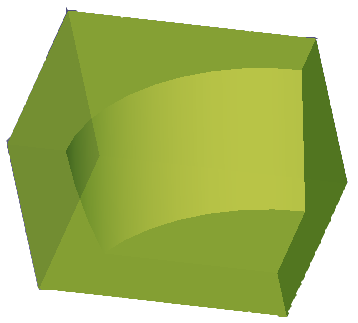
\includegraphics[width=4cm]{tals/stereo/img/aehnlich_klein.png} & 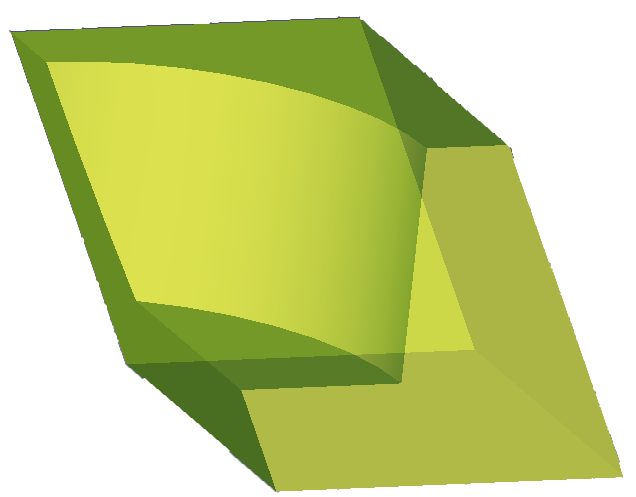
\includegraphics[width=6cm]{tals/stereo/img/aehnlich_gross.png}\\

  \end{tabular} 

Wir bezeichnen im folgenden mit $K$ den Originalkörper und mit $K'$ den gesttreckten, ähnlichen Körper.

Wir erinnern uns an den Streckungsfaktor $k$ der Planimetrie:
\begin{definition}{}{}
  Eine Strecke $a$ wird mit dem
  $$\textrm{Streckungsfaktor} \,\, k$$
  multipliziert, um die Strecke $a'$ im ähnlichen Körper zu erhalten.
\end{definition}

Für $K$ und $K'$ gilt nun:

\begin{gesetz}{}{}
  Der (lineare) Streckungsfaktor sei $k$.

  $$a' = a \cdot{} k^1 = a\cdot{}k $$
  $$A' = A \cdot{} k^2 $$
  $$V' = V \cdot{} k^3 $$
\end{gesetz}

\begin{bemerkung}{Volumina}{}
Der Exponent beim Streckungsfaktor $k$ entspricht der \textbf{Dimension}\index{Dimension!Ähnlichkeit} der
betrachteten «Volumina». Dabei ist das \textbf{zweidimensionale Volumen}\index{Volumen!Ähnlichkeit} die
Fläche während die Streckenlänge das \textbf{eindimensionale Volumen} darstellt.
\end{bemerkung}

\begin{bemerkung}{Verhältnisse}{}
  $$k = \frac{a'}{a} = \sqrt{\frac{A'}{A}} = \sqrt[3\,\,\,]{\frac{V'}{V}}$$
\end{bemerkung}
\newpage


\subsection{Referenzaufgabe Prismen}
Das Verhältnis der Volumina zweier ähnlicher Prismen ist
11:9. Berechnen Sie das Verhältnis der sich entsprechenden Grundflächen und
der sich entsprechenden Seitenlängen.

\TNT{4.0}{$k = \sqrt[3]{\frac{9}{11}}\approx{} 0.9353$. Dies ist
  gleichwohl das Verhältnis der Seitenlängen. Das Verhältnis der
  Flächen erhalten wir, wenn wir $k$ quadrieren $k^2 \approx 0.8748$   }

\subsection{Referenzaufgabe Würfel}
Berechnen Sie die Kantenlänge eines Würfels, dessen Volumen 1dl misst.
\TNT{2.4}{1dl = 0.1 l = 0.1 $\textrm{dm}^3$.
$$\sqrt[3 \,]{0.1 \textrm{dm}^3} = 0.4642\textrm{dm} = 4.642\textrm{cm}$$
}

\TALSGeomAadB{142.ff}{34. [Aufgabe 34. mit TR], 80., 216.}

\newpage
